\chapter{محیط فوتبال ربوکاپ}
در این بخش به معرفی مفاهیم پایه محیط فوتبال ربوکاپ و توصیف چگونگی عملکرد آن می‌پردازیم.
این مفاهیم شامل قوانین بازی، رفتار‌های ممکن، کد پایه ایجنت
، حالت پنالتی، و روش اجرای بازی می‌باشند.
\section{معرفی لیگ}
\subsection{اهداف لیگ}
لیگ ربوکاپ مجموعه مسابقاتی سالانه است که قصد دارد با کمک فوتبال، به پیشرفت زمینه‌های رباتیک و هوش مصنوعی کمک کند.
علت انتخاب فوتبال به عنوان محیط مسابقه، این است که فوتبال یکی از محیط‌هایی است که می‌تواند مسائل مختلفی از جمله تصمیم‌گیری، هماهنگی، بینایی ربات، و ارتباط را در بر داشته باشد.
یکی از اهداف بلندمدت لیگ، ساختن ربات‌هایی است که بتوانند تا سال ۲۰۵۰، تیمی از انسان‌ها را به چالش بکشند.

یکی از لیگ‌های این مسابقات، لیگ شبیه‌ساز فوتبال دو بعدی است.
همانطور که از اسم لیگ پیداست، مسابقه حالت دو بعدی دارد، به این منظور که فضا حالت دید از بالا دارد، و همه حرکات بازیکنان و توپ روی سطح زمین انجام می‌شود.
تمرکز اصلی این لیگ، تصمیم‌گیری و استراتژی، و ساختن الگوریتم‌های مناسب با محیط‌های چند‌عامله با دید ناقص است.
\subsection{ویژگی‌های محیط و قوانین بازی}
مشابه با فوتبال واقعی، هر بازی متشکل از دو تیم ۱۱ نفره است که هر کدام از این نفرات یک عامل مستقل می‌باشد.
بازی در یک مستطیل به ابعاد ۱۱۵ در ۶۸ انجام می‌شود، و هر تیم یک دروازه‌بان دارد که در هر طرف زمین قرار دارد.
بازی در ۶۰۰۰ گام\LTRfootnote{Cycle}
 انجام می‌شود که به دو نیمه تقسیم‌ شده، و هر گام ۱۰۰ میلی‌ثانیه طول می‌کشد. سرور مسابقات در هر گام، اطلاعات مربوط به وضعیت بازی را به تمامی عامل‌ها می‌فرستد، و عامل‌ها باید تصمیم‌گیری خود را بر اساس این اطلاعات انجام دهند.

بازیکنان دید محدودی دارند. با توجه به زاویه گردنی که تنظیم کرده‌اند، یک قطاع از زمین را مشاهده می‌کنند و فقط اطلاعات مربوط به بازیکنان و اشیاء داخل این قطاع را دریافت می‌کنند در شکل \ref{fig:view} نمونه دید یک بازیکن نشان داده شده است.
اطلاعات بازیکنانی که داخل دید نیستند، باید از حافظه بازیکن و یا از ارتباط با سایر بازیکنان به دست آید.
شایان به ذکر است که مشاهدات هر بازیکن، دارای کمی خطای اندازه‌گیری است و به طور کامل دقیق نیست. به طور مشابه، ضربات بازیکن به توپ نیز کمی خطا دارند و کامل دقیق نیستند.

هر عامل باید به صورت مستقل تصمیم‌گیری کند و ارتباط بسیار ناچیزی با سایر عاملین دارد.
در صورتی که دو عامل بخواهند ارتباط برقرار کنند، گیرنده باید از قبل توجه خود را به فرستنده تنظیم کرده‌باشد، و فرستنده حداکثر ۸ بایت می‌تواند ارسال کند.

\begin{figure}[H]
\centering
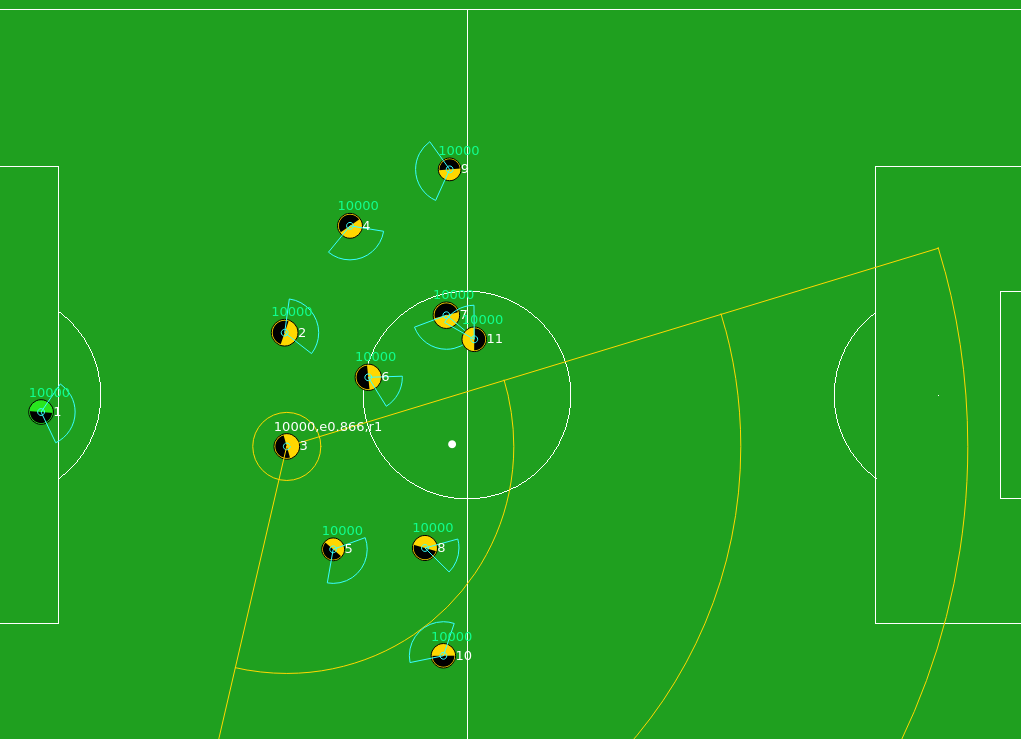
\includegraphics[width=0.75\textwidth]{images/view.png}
\caption{نمونه دید یک بازیکن. در این مثال، بازیکن ۳، بازیکن ۵ و ۸ و ۱۰ و توپ را می‌بیند و از موقعیت سایر بازیکنان اطلاعی ندارد.}\label{fig:view}
    
\end{figure}

هر عامل یک رزرو انرژی و یک منبع انرژی دارد. در صورت پر نبودن انرژی بازیکن، انرژی به نرخ ثابتی از رزرو به منبع منتقل می‌شود.
در صورت اتمام انرژی منبع، رفتار‌های بازیکن از جمله حرکت‌کردن کند‌تر می‌شوند.
رفتار‌های بیشتری (مانند تکل زدن، خطا و ضربه‌ آزاد، کارت زرد و قرمز و ...) 
نیز در محیط به کمک مدل‌های ریاضیاتی پیاده‌سازی شده‌است که خارج از دامنه این پروژه می‌باشد.

\section{کد پایه ایجنت}
در سال‌های اول مسابقات، هر تیمی کد عامل خود را از صفر می‌نوشت، که میزان در دسترس بودن لیگ را بسیار پایین آورده‌بود. با توجه به یکسان بودن بخش عمده‌ای از نیازمندی‌های تیم‌ها،
همچون نیاز به اتصال به سرور، نیاز به تفکیک وظایف بازیکنان به دروازه‌بان و مدافع و مهاجم، نیاز به موقعیت‌یابی اشیا در زمین، توابع هندسی، و ...، هیدهیسا آکیام از تیم هلیوس در سال ۲۰۱۲ تصمیم به ساختن یک کد پایه به صورت متن‌باز محض استفاده سایر تیم‌ها گرفت.
این کد پایه، که کد پایه ایجنت نام دارد، زیربنای ۱۳ تیم از ۱۵ شرکت‌کننده سال اخیر ربوکاپ بوده، و نقطه شروع اکثر کسانی است که قصد فعالیت در این فضا را دارند.
این کد پایه همچنان در حال به‌روز‌رسانی و تقویت‌شدن است
\LTRfootnote{\url{https://github.com/helios-base/helios-base}}
، و خود منشا سایر کد پایه‌های به اشتراک گذاشته‌شده همچون کد پایه گلایدرز\LTRfootnote{Gliders}
 و کد پایه سایرس\LTRfootnote{Cyrus}
  است.

با استفاده از این کد پایه، توسعه‌دهندگان می‌توانند سطح کدزدن خود را از سطوح پایین، به سطح استراتژی و تاکتیک و تصمیم‌گیری منتقل کنند. به طور مثال
بدون استفاده از یک کد پایه، برای حرکت عامل به مرکز زمین باید کد اتصال به سرور و موقعیت‌یابی را پیاده‌سازی کنیم. سپس درگیر مسائلی همچون محاسبه شتاب بازیکن، نیرویی که باید اعمال شود، مسیر حرکت بهینه (چرخیدن و دویدن یا دویدن مورب)
 و ... شوند. در حالی که این عمل، به صورت یک دستور سطح بالا در کد پایه ایجنت قابل اجراست. در بخش بعدی به تمام رفتار‌های ممکن در این کد پایه و سطح‌بندی رفتار‌ها می‌پردازیم.

\section{معرفی رفتار‌های ممکن}
هر عامل در هر لحظه، باید تصمیم‌گیری خود را به سرور بفرستد.
این تصمیم‌گیری می‌تواند شامل انجام یکی از رفتار‌های ممکن باشد.
در هر لحظه، عامل می‌تواند گردن خود را بچرخاند تا اطراف خود را ببیند، و همزمان یکی از پنج رفتار ضربه به توپ، حرکت بدن، چرخش بدن، تکل، یا گرفتن توپ را انجام دهد.
رایج است که رفتار‌های ممکن و پیاده‌سازی شده را به سه طبقه تقسیم‌بندی کنیم که در پایین‌ترین سطح، رفتار‌های سطح‌ سرور، و در بالا‌ترین سطح، رفتار‌های سطح استراتژیک و فکری
قرار می‌گیرند.
\subsection{رفتار‌های سطح پایین}
در پایین‌ترین سطح، رفتار‌ها مستقیما معادل با رفتار‌های مورد پذیرش سرور می‌باشند.
این رفتار‌ها شامل اعمال نیرو روی توپ در یک راستا (نسبت به بدن بازیکن)
 و نیروی خاص، 
 چرخاندن بازیکن به یک راستا،
اعمال نیروی حرکت بازیکن در راستا و نیرو،
تکل زدن در یک راستا،
و گرفتن توپ (در صورتی که بازیکن دروازه‌بان باشد)
می‌باشند.

\subsection{رفتار‌های سطح متوسط}
در این سطح، رفتار‌ها ساده‌سازی شده‌اند تا استفاده‌ از آن‌ها برای تصمیم‌گیری راحت‌تر باشد. 
به طور مثال رفتار حرکت به سمت یک نقطه‌ خاص از زمین،
رفتار ضربه زدن به توپ با سرعت دلخواه در راستای غیرنسبی،
رفتار ضربه زدن توپ به صورت چند‌ضرب به یک نقطه خاص،
و...
را می‌توان از رفتار‌های این سطح معرفی کرد.
\subsection{رفتار‌های سطح بالا}
در این سطح، رفتار‌ها حالت استراتژی و فکر کردن دارند، و به صورت انتزاعی و مشابه با فوتبال واقعی می‌باشند.
به طور مثال، حرکت به سمت نقطه‌ی آرایش\LTRfootnote{Formation}،
حرکت برای قطع توپ،
زدن شوت (در صورت ممکن بودن شوت موفق)،
و...
از رفتار‌های سطح بالا می‌باشند.
\section{حالت دید کامل}
همانطور که گفته‌شد، محیط اطلاعات کامل را در اختیار عامل قرار نمی‌دهد. با توجه به اینکه قصد تغییر کد سرور مسابقات و افزودن پاداش به سرور را نداریم، این محاسبات درون خود عامل باید صورت بگیرند.
خوش‌بختانه سرور مسابقات قابلیت ارسال محیط در حالت دید کامل
\LTRfootnote{Fullstate WorldModel}
 را دارد که در این حالت، همه اطلاعات بدون نویز به عامل ارسال می‌شوند.
 داخل کد ایجنت می‌توان انتخاب کرد که در صورت دریافت حالت دید کامل آن‌را جایگزین دید ناقص کند، یا اینکه هر دو را کنار هم نگه‌دارد.
 ما در فرآیند یادگیری تقویتی از حالت دوم استفاده می‌کنیم تا با کمک دید کامل محاسبات پاداش را انجام دهیم، و با حالت دید ناقص تصمیم‌گیری کنیم.
در عکس \ref{fig:ss2d_rl_loop} می‌توان مشاهده کرد که پاداش داخل عامل محاسبه‌شده، و تابعی از حالت دید کامل (\lr{Fullstate} یا به اختصار \lr{FS})
است، و محیط هر دو حالت دید را برای عامل ارسال می‌کند.
این نمودار در واقع حالت اصلاح‌شده \ref{fig:agent_env} است که خاص‌منظوره این پروژه می‌باشد.
 \begin{figure}[H]
    \centering
    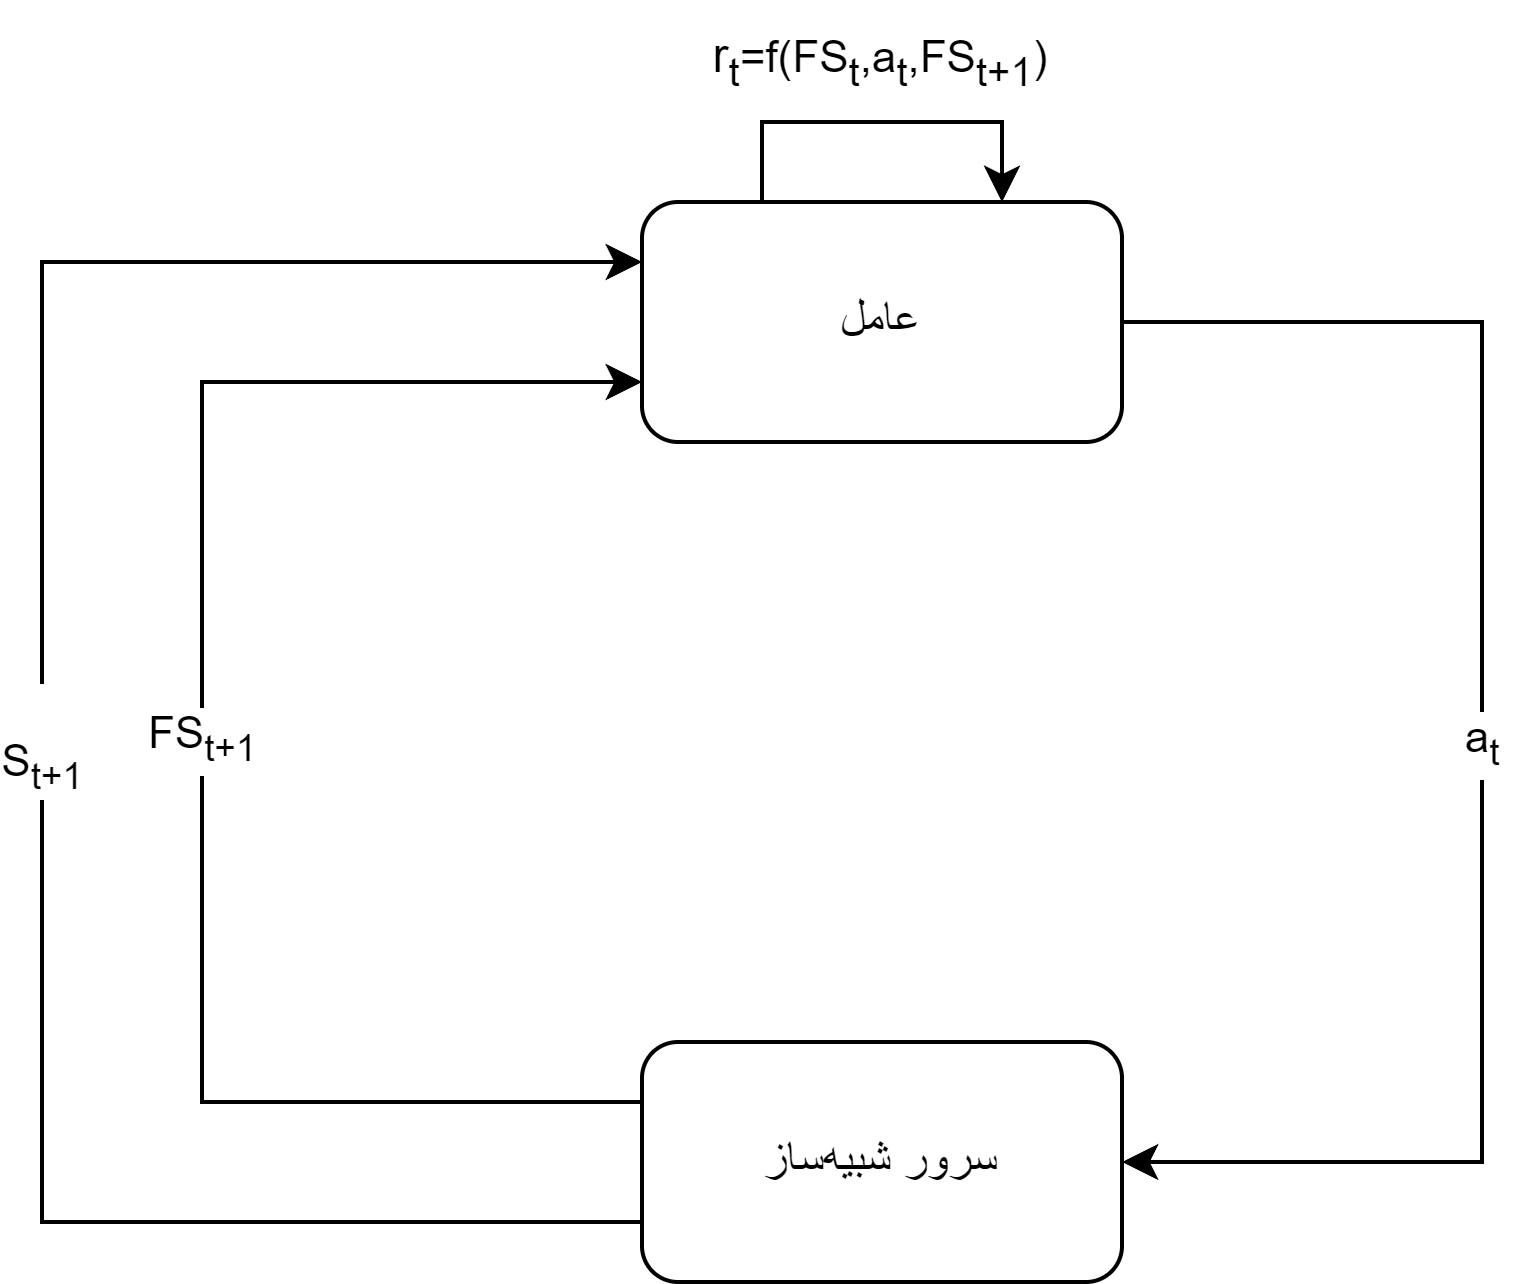
\includegraphics[width=0.75\textwidth]{images/ss2d_reward.png}
    \caption{ارتباط بین محیط و عامل، و روش محاسبه پاداش}\label{fig:ss2d_rl_loop}
 \end{figure}
\section{معرفی حالت پنالتی}
در صورت تساوی بازی در ده دقیقه زمان عادی، و تداوم تساوی پس از وقت اضافی، بازی به حالت پنالتی می‌رود. 
با توجه به دو بعدی بودن محیط، در صورتی که مشابه با فوتبال واقعی، پنالتی به صورت تک ضرب باشد، می‌توان برای آن استراتژی قطعی ارائه داد.
به همین منظور، پنالتی در فضای لیگ دو‌بعدی، به صورت تک به تک با دروازه‌بان است.

بازیکن مهاجم، ۱۵ ثانیه فرصت دارد تا توپ را به گل تبدیل کند. دروازه‌بان باید در این مدت تلاش کند جوری موقعیت‌گیری کند که حریف نتواند شوت منجر به گل داشته‌باشد.
در صورتی که زمان مهاجم تمام شود، توپ به بیرون محیط بازی برود، یا توپ توسط دروازه‌بان گرفته‌شود، دروازه‌بان برنده می‌شود. در صورتی که توپ وارد گل شود، مهاجم برنده می‌شود.

با توجه به تک‌عامله بودن، و محدود بودن زمان محیط، می‌توان از روش‌های یادگیری تقویتی برای یادگیری استراتژی‌های بهینه برای پنالتی استفاده کرد.
در شکل
\ref{fig:penalty_demo}
 یک نمونه از حالت پنالتی را مشاهده می‌کنید.
\begin{figure}[H]
\centering
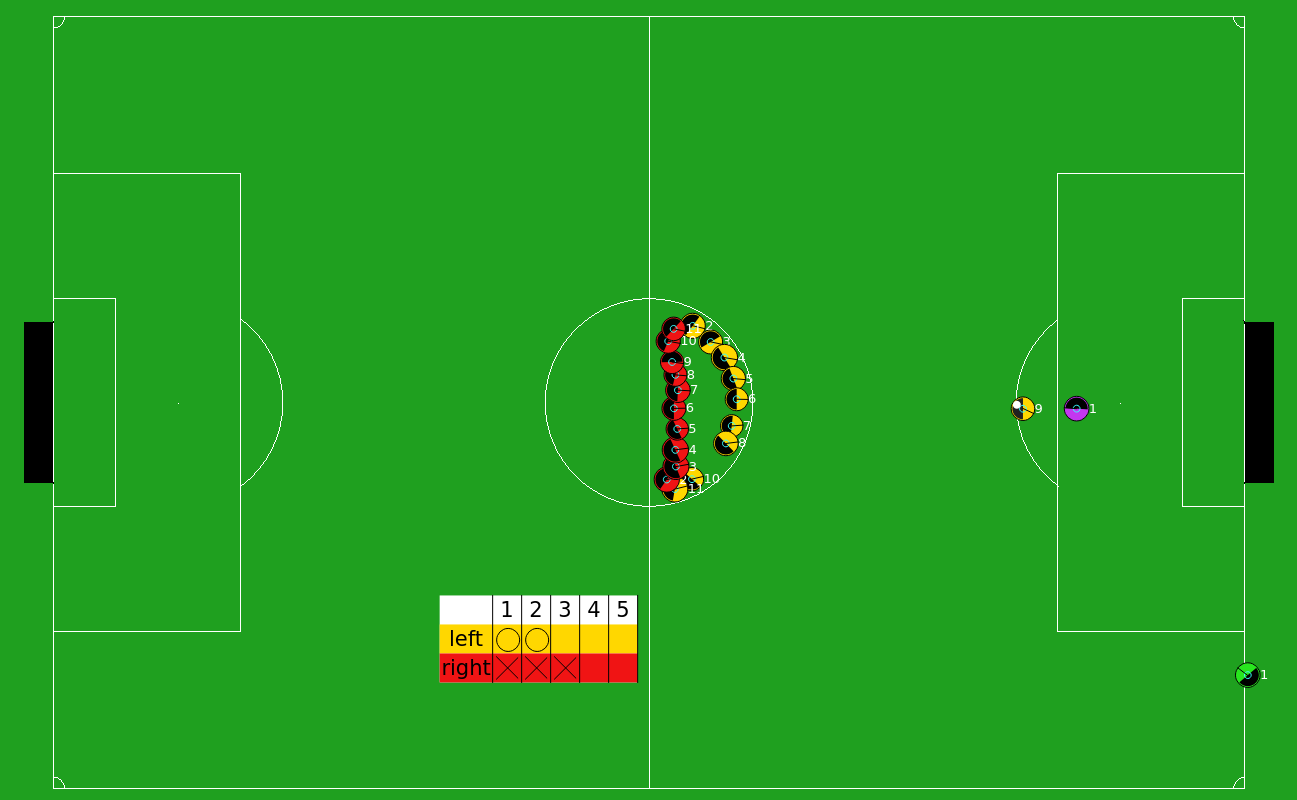
\includegraphics[width=0.75\textwidth]{images/penalty.png}
\caption{نمونه‌ای از بازی در حالت پنالتی}\label{fig:penalty_demo}
\end{figure}
\section{کار با مربی تمرینی برای تولید محیط‌ قابل تکرار}
با توجه به اینکه برای یادگیری تقویتی، نیاز به بازگرداندن محیط به حالت اولیه را داریم، می‌توانیم از 
مربی تمرینی\LTRfootnote{Trainer}
استفاده کنیم.
در صورتی که در تنظیمات سرور، این حالت فعال شده باشد، می‌توان کدی نوشت که در شرایط دلخواه، توپ و بازیکنان را جا‌به‌جا کنیم،
حالت بازی را تنظیم کنیم، انرژی بازیکنان را پر کنیم‌ و ... .
در فصل‌های آینده از این امکان، برای ساختن یک رابط استاندارد یادگیری تقویتی برای محیط فوتبال استفاده خواهیم کرد.
\section{جمع‌بندی}
در این فصل، محیط فوتبال ربوکاپ دوبعدی به عنوان یک ابزار مطالعاتی برای تقویت پیشرفت‌ها در زمینه هوش مصنوعی و رباتیک معرفی شد.
این محیط، با ارائه یک پلتفرم مسابقه‌ای مبتنی بر قوانین فوتبال واقعی، فرصت‌هایی برای توسعه و آزمایش الگوریتم‌های تصمیم‌گیری، هماهنگی، و استراتژی در محیط‌های چندعامله فراهم می‌کند.

معرفی این محیط شامل توضیح قوانین بازی، نحوه ارتباط و تصمیم‌گیری عامل‌ها، و همچنین ساختار کد پایه ایجنت بود که توسعه‌دهندگان را قادر می‌سازد تا تمرکز خود را بر روی تاکتیک و تصمیم‌گیری‌های سطح بالای مشابه با فوتبال معطوف دارند.

یکی از نوآوری‌های کلیدی در این فصل، استفاده از حالت دید کامل در کنار دید ناقص است که به عامل‌ها امکان می‌دهد تا پاداش‌ها را بر اساس اطلاعات کامل محیط محاسبه کنند، در حالی که تصمیم‌گیری بر اساس دید ناقص انجام می‌شود. این رویکرد یک قدم مهم در راستای افزایش قابلیت‌های یادگیری تقویتی در محیط‌هایی با دید ناقص است.

همچنین، با معرفی حالت پنالتی و استفاده از مربی تمرینی برای تولید محیط‌های قابل تکرار، زمینه‌های لازم برای پیاده‌سازی الگوریتم‌های یادگیری تقویتی فراهم شده است. این امکانات به پژوهشگران اجازه می‌دهد تا در یک محیط مسابقه‌ای استاندارد، استراتژی‌های بهینه‌سازی شده را آزمایش و توسعه دهند.